\documentclass[10pt, aspectratio=169]{beamer}

\usetheme[progressbar=frametitle]{metropolis}
\usecolortheme{tse}

\usepackage{appendixnumberbeamer}

\usepackage{booktabs,natbib,adjustbox}
\usepackage[scale=2]{ccicons}

\usepackage{pgfplots}
\usepgfplotslibrary{dateplot}

\usepackage{xspace}
\newcommand{\themename}{\textbf{\textsc{metropolis}}\xspace}

% \renewcommand{\familydefault}{\sfdefault}
\newcommand{\indep}{\perp\!\!\!\!\perp} % the independent symbol
\usepackage{bbm}
% % define theorem
% \newtheorem{theorem}{Theorem}[section]
% \newtheorem{corollary}[theorem]{Corollary}
% \newtheorem{assumption}{Assumption}[subsection]
% define definition style
% \theoremstyle{definition}
% \newtheorem{definition}{Definition}[section]
% \newtheorem{proposition}{Proposition}[section]
% \newtheorem{property}{Property}[section]
% \newtheorem{example}{Example}[section]
% \newtheorem*{exercise}{Exercise}
% % define remark style
% \theoremstyle{remark}
% \newtheorem*{remark}{Remark}
% \newtheorem{question}{Question}
% \newenvironment{sol}{\begin{proof}[Solution]}{\end{proof}}

\newcommand{\R}{\mathbb{R}}
\newcommand{\C}{\mathbb{C}}
\newcommand{\Rd}{\mathbb{R}^d}
\newcommand{\Hy}{\mathbb{H}}
\newcommand{\calh}{\mathcal{H}}
\newcommand{\cala}{\mathcal{A}}
\newcommand{\calm}{\mathcal{M}}
\newcommand{\cald}{\mathcal{D}}
\newcommand{\caln}{\mathcal{N}}
\newcommand{\calr}{\mathcal{R}}
\newcommand{\calz}{\mathcal{Z}}
\newcommand{\caly}{\mathcal{Y}}
\newcommand{\calq}{\mathcal{Q}}
\newcommand{\cale}{\mathcal{E}}
\newcommand{\cali}{\mathcal{I}}
\newcommand{\calb}{\mathcal{B}}
\newcommand{\calc}{\mathcal{C}}
\newcommand{\calw}{\mathcal{W}}
\newcommand{\calg}{\mathcal{G}}
\newcommand{\calu}{\mathcal{U}}
\newcommand{\calo}{\mathcal{O}}
\newcommand{\calp}{\mathcal{P}}
\newcommand{\vect}{\mathrm{vect}}
\newcommand{\cov}{\mathrm{cov}}
\newcommand{\reff}{\mathrm{ref}}

\newcommand{\setbra}[1]{\left\{#1\right\}}
\newcommand{\set}[1]{\setbra{#1}}
\newcommand{\bra}[1]{\left[#1\right]}
\newcommand{\pa}[1]{\left(#1\right)}
\newcommand{\abs}[1]{\left| #1\right|}
\newcommand{\norm}[1]{\left\| #1 \right\|}
\newcommand{\angs}[1]{\left\langle #1\right\rangle}
\newcommand{\midvert}{\middle|}

\newcommand{\Q}{\mathbb{Q}}
\newcommand{\Lip}{\mathrm{Lip}}
\newcommand{\Z}{\mathbb{Z}}
\newcommand{\N}{\mathbb{N}}
\newcommand{\Cpx}{\mathbb{C}}
\newcommand{\E}{\mathbb{E}}
\newcommand{\V}{\mathbb{V}}
\newcommand{\Var}{\mathrm{Var}}
\newcommand{\p}{\mathbb{P}}
\newcommand{\F}{\mathcal{F}}
%\newcommand{\G}{\mathcal{G}}
\newcommand{\diag}{\mathrm{diag}}
\newcommand{\id}{\mathrm{id}}
\newcommand{\one}{\mathbbm{1}}
\newcommand{\defeq}{\overset{\mathrm{def}}{=}}
\newcommand{\nlr}{\nleftrightarrow}
\newcommand{\lr}{\leftrightarrow}
\newcommand{\ra}{\rightarrow}
\newcommand{\tr}{\mathrm{tr}}
\newcommand{\pspace}{(\Omega, \F, \p)}
\newcommand{\filt}{\pa{\F_t}_{0\leq t\leq \infty}}
\newcommand{\filtnat}{\pa{\F_t^X}_{0\leq t\leq \infty}}
\newcommand{\filtspace}{\pa{\Omega, \F, \filt, \p}}
\newcommand{\indist}[1]{\overset{d}{#1}}
\newcommand{\inlo}[1]{\overset{L^1}{#1}}
\newcommand{\inltwo}[1]{\overset{L^2}{#1}}
\newcommand{\inp}[1]{\overset{\p}{#1}}
\newcommand{\inpc}{\overset{\p}{\rightarrow}}
\newcommand{\indistc}{\indist{\rightarrow}}
\newcommand{\inas}[1]{\overset{\mathrm{a.s.}}{#1}}
\newcommand{\inhy}[1]{\overset{\mathrm{\Hy^2}}{#1}}
\newcommand{\cc}[1]{\mathrm{CC}\left(#1 \right)}
\newcommand{\partfrac}[1]{\frac{\partial}{\partial #1}} \newcommand{\Chi}{\mathcal{X}} \newcommand{\tl}{{T,\Lambda}}
\newcommand{\isingspace}{\{\pm\}^\Lambda} \newcommand{\boltzmeas}{\mu_\tl}
\newcommand{\bl}{{\beta, \Lambda}} \newcommand{\zerot}{{t\in [0,T]}}
\newcommand{\tgez}{{t\geq 0}} \newcommand{\brown}{(B_t)_\tgez}
\newcommand{\process}{(X_t)_\tgez} \newcommand{\smallising}[4]{\begin{matrix} #1&#2\\#3&#4\end{matrix}}
\def\ci{\perp\!\!\!\!\perp}
\newcommand{\parm}{{(m)}} \newcommand{\diff}{\mathrm{d}} \newcommand{\optp}{\mathrm{opt}_\p}
\newcommand{\erp}{\mathrm{er}_\p} \newcommand{\er}{\mathrm{er}}
\newcommand{\sgn}{\mathrm{sgn}} \DeclareMathOperator*{\argmin}{arg\,min}
\DeclareMathOperator*{\argmax}{arg\,max}
\DeclareMathOperator*{\esssup}{ess\,sup}
\DeclareMathOperator*{\essinf}{ess\,inf} \newcommand{\vcdim}{\mathrm{VCdim}}
\newcommand{\bigargs}{\pa{\bar{Y}_t,M_t,\theta_t}}
\newcommand{\bigargsm}{\pa{\bar{Y}_{t-},M_{t-},\theta_{t-}}}
\newcommand{\smallargs}{\pa{\bar{y},m,\vartheta}}
\newcommand{\smallarg}{\pa{m,\vartheta}}

\newcommand{\fatone}{\mathbf{1}}
\newcommand{\pen}{\mathrm{pen}}
\newcommand{\MF}{\mathrm{MF}}
\newcommand{\opt}{\mathrm{opt}}
\newcommand{\MSE}{\mathrm{MSE}}
\newcommand{\MISE}{\mathrm{MISE}}
\newcommand{\CV}{\mathrm{CV}}

\newcommand{\1}{\mathbbm{1}}


\newcommand\footlineon{
  \setbeamertemplate{footline} {
    \begin{beamercolorbox}[ht=2.5ex,dp=1.125ex,leftskip=.8cm,rightskip=.6cm]{structure}
      \footnotesize \insertsection
      \hfill
      {\insertframenumber}
    \end{beamercolorbox}
    \vskip 0.45cm
  }
}
\footlineon

% \metroset{sectionpage=none}

\title{Optimal Urban Transportation Policy}
\subtitle{Evidence from Chicago}
\date{Presented by Zixuan}
\author{Milena Almagro, Felipe Barbieri, Juan Camilo Castillo, Nathaniel Hickok, Tobias Salz}
\institute{\today}
% \titlegraphic{\hfill\includegraphics[height=1.5cm]{logo.pdf}}

\begin{document}

\maketitle

% \begin{frame}{Table of contents}
%   \setbeamertemplate{section in toc}[sections numbered]
%   \tableofcontents%[hideallsubsections]
% \end{frame}
\begin{frame}{Motivation}
  \begin{figure}
    \centering
    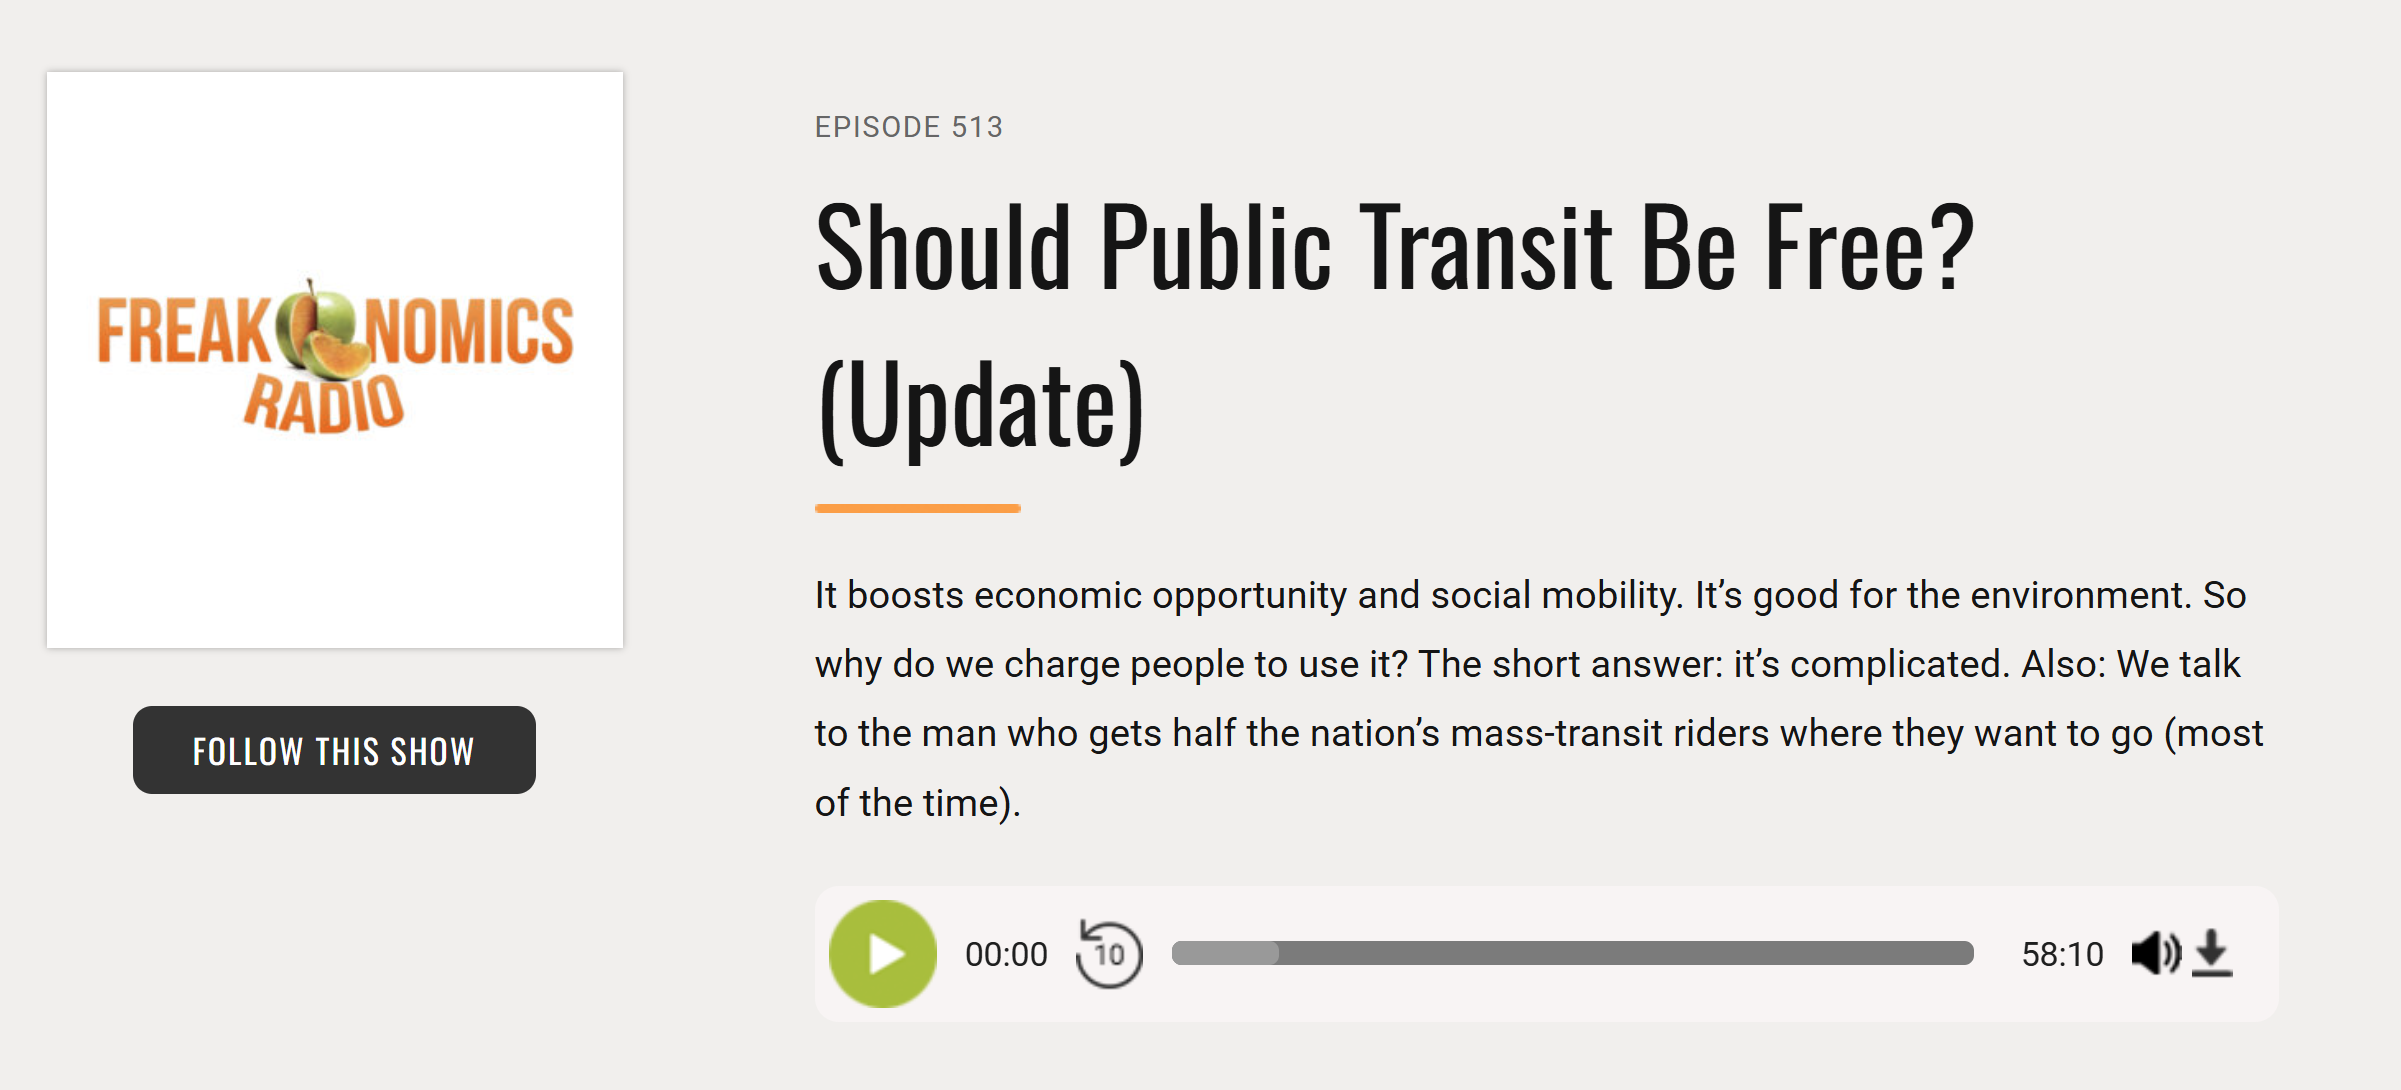
\includegraphics[width=\textwidth]{../Figures/freakonomics_2.png}
  \end{figure}
\end{frame}

\begin{frame}{Motivation}
  When it comes to transportation policy,
  \begin{itemize}
    \item Free public transit?
    \item High quality service?
    \item Road pricing (cordon tax)?
  \end{itemize}
\end{frame}

\section{Introduction}
\begin{frame}{Transportation Policy}
  We consider three modes of transportation:
  \begin{itemize}
    \item \textbf{Public transit}: \textbf{fare $p$, frequency $k$}
          \begin{itemize}
            \item Train/Metro
            \item Bus
          \end{itemize}
    \item Driving: \textbf{road pricing $p$}
    \item Ride hailing (taxi, uber): fare $p$
  \end{itemize}
  \begin{block}{Question}
    Assuming that the government has control over the \textbf{public transit} and \textbf{road pricing}, what is the optimal price $p$ and quality $k$ that maximizes \textbf{social welfare}, while taking into account \textbf{environmental costs} and \textbf{budget constraint}?
  \end{block}
\end{frame}

\begin{frame}{Optimal Policy}
  For each transportation mode, define
  \begin{itemize}
    \item $p_j$: the price (fare, road tax etc.)
    \item $k_j$: the frequency (quality measure)
    \item $q_j$: the total demand for mode $j$
    \item $t_j$: the time spent on mode $j$
  \end{itemize}
  The social welfare function $U(p,t)-C(q,k)-E(q,k)$ consists of three components:
  \begin{itemize}
    \item Gross utility: $U(p,t)$
    \item Cost of proving the service: $C(q,k)$
    \item Environmental cost: $E(q,k)$
  \end{itemize}

\end{frame}

\begin{frame}{Optimal Policy}
  The budget constraint is giveN by
  \begin{equation*}
    B+\sum_{j\in G} (p_j q_j - C_j)\ge 0
  \end{equation*}
  \begin{block}{Problem}
    The optimal transportation policy is essentially solving for the set of \alert{ prices $p$ and frequencies $k$} of the following the constrained problem
    \begin{equation*}
      \begin{split}
        \max_{p_j,k_j} & \quad U(p,t)-C(q,k)-E(q,k)                 \\
        \text{s.t.}    & \quad B+\sum_{j\in G} (p_j q_j - C_j)\ge 0
      \end{split}
    \end{equation*}
  \end{block}
\end{frame}
\section{Model}
\begin{frame}{Demand side $q(p,t)$}
  A traveler with type $\theta$ chooses mode $j^*$ such that
  \begin{equation*}
    j^*(\theta) = \argmax_{j \in \mathcal{J}(\theta) \cup \{0\}} u_j(t_j, \theta) - p_j
  \end{equation*}
  Explicitly,
  \begin{equation*}
    \max_{j \in \mathcal{J}_m^i \cup \{0\}} \xi_{mj} + \alpha_T \cdot T_{mj} + \alpha_p^i \cdot p_{mj} + \epsilon_{mj}^i
  \end{equation*}
  The choice probability is given by
  \begin{equation*}
    \p_{mj}^i = \frac{\exp\left( \frac{\delta_{mj}^i}{1-\rho} \right)}{
      \left[ \sum_{j \in g} \exp\left( \frac{\delta_{mj}^i}{1-\rho} \right) \right]^\rho \cdot \left( \sum_g \left[ \sum_{j \in g} \exp\left( \frac{\delta_{mj}^i}{1-\rho} \right) \right]^{(1-\rho)} \right)}
  \end{equation*}
\end{frame}

\begin{frame}{Demand side $q(p,t)$}
  Given vectors of $p$ and $t$, demand for mode $j$ is given by
  \begin{equation*}
    q_j = q_j({p}, {t}) = \int_{\Theta_j({p}, {t})} f(\theta) d\theta
  \end{equation*}
  Explicitly,
  \begin{equation*}
    \p_{mj} = \int \p_{mj}^i \, dF_m(\alpha_p^i),
    \quad q_{mj} = N_m \cdot \p_{mj}
  \end{equation*}
\end{frame}

\begin{frame}{Demand side $q(p,t)$}
  Gross utility is given by the sum of each mode's utility
  \begin{equation*}
    U(p,t) = \sum_{j\in J} \int_{\Theta_j(p,t)} u_j(t_j,\theta) f(\theta) d\theta
  \end{equation*}
  \begin{block}{Demand \& Supply}
    Demand can be written as a function of price $p$ and travel time $t$. That is,
    \begin{equation*}
      q = q(p,t)
    \end{equation*}
    However note that travel time $t$ is not exogenously given. It is affected by
    the demand $q$ as well as the frequency $k$. That is,
    \begin{equation*}
      t = t(p,k)
    \end{equation*}
  \end{block}

\end{frame}

\begin{frame}{Supply side $t(p,k)$}
  To make the travel time function explicit,
  \begin{equation*}
    T_{mj} = \gamma \cdot \left( T_{mj}^{\text{walk}} + T_{mj}^{\text{wait}} \right) + T_{mj}^{\text{vehicle}}
  \end{equation*}
  % The in vehicle time at time $h$ for edge $e$ is given by
  % \begin{equation*}
  %   T_{ehj}^{\text{vehicle}} = \max \left\{ T_{ej}^0, A_{ehj} \cdot F_{eh}^{\beta_j} \right\}
  % \end{equation*}
  % Thus, the total in vehicle time is
  % \begin{equation*}
  %   T_{mj}^{\text{vehicle}} = \sum_{e \in P_{mj}} T_{ehj}^{\text{vehicle}}
  % \end{equation*}
  For waiting time,
  \begin{itemize}
    \item public transit: taking into account the reliability
    \item ride hailing: taking into account idle drivers in the vicinity
  \end{itemize}
  For in vehicle time, it takes into account \textbf{congestion}. When the total flow of vehicle on an edge is
  \begin{itemize}
    \item  below a certain threshold: the in vehicle time is the \textit{free flow} time
          suggested by Google Maps.
    \item above: a function of the total flow on the edge.
  \end{itemize}
\end{frame}
\begin{frame}{Equilibrium $q$ \& $t$}
  \begin{block}{Equilibrium}
    Given price $p$ and frequency $k$, an equilibrium is a vector of $q$ and $t$
    such that
    \begin{equation*}
      q = q(p,t), \quad t = t(p,k)
    \end{equation*}
  \end{block}
  Solving the equilibrium is essentially finding the fixed point of the function
  \begin{equation*}
    f_{p,k}(q)=q(p,t(p,k))
  \end{equation*}
  The author uses a limited-memory version of Broyden's method to find the root of $f_{p,k}(q)-q=0$.
\end{frame}
\begin{frame}{Recap}
  \begin{enumerate}
    \item The optimal policy $p^*, k^*$ is derived from iteratively maximizing problems
          that approximate the Lagrangian of the main problem.
    \item Every evaluation of the Lagrangian requires solving for the equilibrium $q^*$
          and $t^*$.
  \end{enumerate}
\end{frame}
\section{Estimation}
\begin{frame}{Demand: endogeneity}
  Recall
  $$ U_{mj}^i = \xi_{mj} + \alpha_T \cdot T_{mj} + \alpha_p^i \cdot p_{mj} + \epsilon_{mj}^i $$
  where $\alpha_p^i = \frac{\alpha_p}{y_i^{1 - \alpha_{py}}}$ and $\xi_{mj} $ is the unobserved demand shock.
  \begin{itemize}
    \item Endogeneity of price: the price for ride hailing is endogenous, while assuming
          that the price of public transit and driving is exogenous to $\xi_{mj}$.
    \item Endogeneity of travel time: higher $\xi_{mj}$ is associated with higher travel
          time. If this source of endogeneity is not addressed, the time coefficient is
          biased towards 0.
  \end{itemize}
\end{frame}

\begin{frame}{Demand: moment condition 1}
  We have two types of moment conditions.\\
  The first one targets the price coefficient $\alpha_p$.
  % We use the price variation introduced by a ride-hailing
  % surcharge that applies to weekday trips that either originate or end in a downtown zone between 6 am and 10 pm. 
  \begin{equation*}
    \mathbb{E} \left[ (\hat{\eta}_{mj} - \tilde{\eta}_{mj}) \mathbbm{1}\{ j = \text{ride-hail}, m \in \mathcal{M}_{\tau} \} \right] = 0
  \end{equation*} where \(\hat{\eta}_{mj}\) is the ride-hailing elasticity from our differences-in-differences estimate (Appendix B), \(\tilde{\eta}_{mj}\) is the model-implied elasticity, and \(\mathcal{M}_{\tau}\) are the markets affected by the surcharge policy.

\end{frame}

\begin{frame}{Demand: moment condition 2}
  The second one targets the travel time coefficient $\alpha_T$ and substitution parameter $\rho$.
  \begin{enumerate}
    \item instrument for travel time: free-flow time $T_{mj}^0$ which do not depend on
          the vehicle flow and therefore not affected by within day demand shock.
    \item instrument for the substitution parameter $\rho$: \citet{gandhi2019measuring}
          \begin{equation*}
            \mathbb{E} \left[ \mathbf{Z}_{mj} \xi_{mj} \right] = 0
          \end{equation*}
  \end{enumerate}
\end{frame}
\begin{frame}
  \begin{table}[htpb]\fontsize{6pt}{6pt}\selectfont
    \centering
    \caption{Demand estimation results}
    
\begin{tabular}{lccccccc}
    \toprule
                        & \multicolumn{5}{c}{Pooled} & \multicolumn{2}{c}{Peak/Off-Peak}                                                                  \\
    \cmidrule(lr){2-6} \cmidrule(lr){7-8}
                        & (1)                        & (2)                               & (3)        & (4)        & (5)        & Peak       & Off-peak   \\
    \midrule
    $\alpha_T$          & -1.068                     & -1.692                            & -2.345     & -2.415     & -1.928     & -1.824     & -1.872     \\
                        & (0.011)                    & (0.022)                           & (0.023)    & (0.023)    & (0.018)    & (0.022)    & (0.027)    \\
    $\alpha_p$          & -0.058                     & -0.155                            & -8.461     & -3.416     & -2.078     & -2.388     & -1.657     \\
                        & (0.001)                    & (0.002)                           & (0.492)    & (0.111)    & (0.09)     & (0.225)    & (0.068)    \\
    $\alpha_{py}$       & .                          & .                                 & -1.262     & -0.588     & -0.414     & -0.696     & -0.152     \\
                        & .                          & .                                 & (0.039)    & (0.02)     & (0.022)    & (0.048)    & (0.022)    \\
    $\rho$              & .                          & .                                 & .          & .          & 0.262      & 0.376      & 0.162      \\
                        & .                          & .                                 & .          & .          & (0.012)    & (0.017)    & (0.017)    \\
    \midrule
    Estimator           & OLS                        & IV                                & GMM        & GMM        & GMM        & GMM        & GMM        \\
    Policy Moment       &                            &                                   & \checkmark & \checkmark & \checkmark & \checkmark & \checkmark \\
    Car Ownership       &                            &                                   &            & \checkmark & \checkmark & \checkmark & \checkmark \\
    Nest                &                            &                                   &            &            & \checkmark & \checkmark & \checkmark \\
    Avg. VOT            & 18.41                      & 10.89                             & 23.88      & 14.65      & 13.47      & 19.47      & 9.81       \\
    VOT (Bot. Quintile) & .                          & .                                 & 2.44       & 3.26       & 3.62       & 3.9        & 3.42       \\
    VOT (Top Quintile)  & .                          & .                                 & 64.24      & 32.36      & 27.94      & 45.32      & 18.09      \\
    Avg. Price Elast.   & -0.2                       & -0.53                             & -0.5       & -0.61      & -0.65      & -0.55      & -0.72      \\
    Avg. Time Elast.    & -0.58                      & -0.91                             & -1.26      & -1.27      & -1.29      & -1.44      & -1.07      \\
    M                   & 92,284                     & 92,284                            & 91,908     & 91,561     & 91,561     & 42,989     & 48,572     \\
    N                   & 281,755                    & 281,755                           & 281,042    & 280,185    & 280,185    & 136,337    & 143,848    \\
    \bottomrule
\end{tabular}


  \end{table}

  % \footnotesize{Notes: This table presents demand estimation results from the specifications outlined in section 4.1. We obtain the average VOT by first computing the within market average VOT as the weighted average of $\alpha_T / \alpha_p^i$ and then averaging across markets, with weights given by market size. Average elasticities are computed as the weighted average of own-price and own-time elasticities across all mode-market observations, with weights given by market size. {We drop markets without income information in specifications with income heterogeneity.}}
\end{frame}
\begin{frame}{Supply: in vehicle time}
  The estimation equation is
  \begin{equation*}
    \log T_{ehj}^{\text{vehicle}} = a_e + \beta_j \log F_{eh} + \epsilon_{ehj}
  \end{equation*}
\end{frame}
\begin{frame}
  \begin{table}[htpb]\fontsize{6pt}{6pt}\selectfont
    \centering
    \caption{Traffic congestion estimation results}
    
\begin{tabular}{lcccccc}
    \toprule
                     & \multicolumn{3}{c}{Bus} & \multicolumn{3}{c}{Car}                                                     \\
    \cmidrule(lr){2-4} \cmidrule(lr){5-7}
                     & (1)                     & (2)                     & (3)        & (4)        & (5)        & (6)        \\
    \midrule
    Log Flow         & 0.092***                & 0.059***                & 0.101***   & 0.128***   & 0.100***   & 0.168***   \\
                     & (0.006)                 & (0.006)                 & (0.008)    & (0.005)    & (0.005)    & (0.004)    \\
    \midrule
    Edge FE          & \checkmark              & \checkmark              & \checkmark & \checkmark & \checkmark & \checkmark \\
    Weather controls &                         & \checkmark              & \checkmark &            & \checkmark & \checkmark \\
    IV               &                         &                         & \checkmark &            &            & \checkmark \\
    within $R^2$     & 0.093                   & 0.129                   & 0.116      & 0.411      & 0.529      & 0.443      \\
    First-stage F    &                         &                         & 2767.096   &            &            & 4487.258   \\
    Observations     & 7962                    & 7962                    & 7962       & 11739      & 11739      & 11739      \\
    \bottomrule
\end{tabular}

  \end{table}

  % \footnotesize{Notes: Standard errors are in parentheses. *** indicates significance at the 1\% level. The dependent variable is the log of travel time in traffic.}
\end{frame}

\begin{frame}{Recap}
  \begin{enumerate}
    \item Estimate demand side parameters $\theta$ to get $q(p,t)$
    \item Estimate supply side/congestion parameters $\beta$ to get $t(p,k)$
    \item Solve the optimal policy $p^*$ and $k^*$.
    \item Compare the welfare under the status quo and the optimal policy.
  \end{enumerate}
\end{frame}
\section{Results}
\begin{frame}{Theoretical results}
  The social planner's problem can be rewritten as the Lagrangian
  \begin{equation*}
    \mathcal{L}(p,k,\lambda)  =U(p,t(q,k))-C(q,k)-E(q,k)+\lambda\pa{B+\sum_{j\in G} (p_j q_j - C_j(q_j,k_j))}
  \end{equation*}
  where $q^*$ is determined by the equilibrium condition $f_{p,k}(q)-q=0$ (implicit function of $p$ and $k$).
\end{frame}

\begin{frame}{Theoretical results}
  \begin{figure}
    \centering
    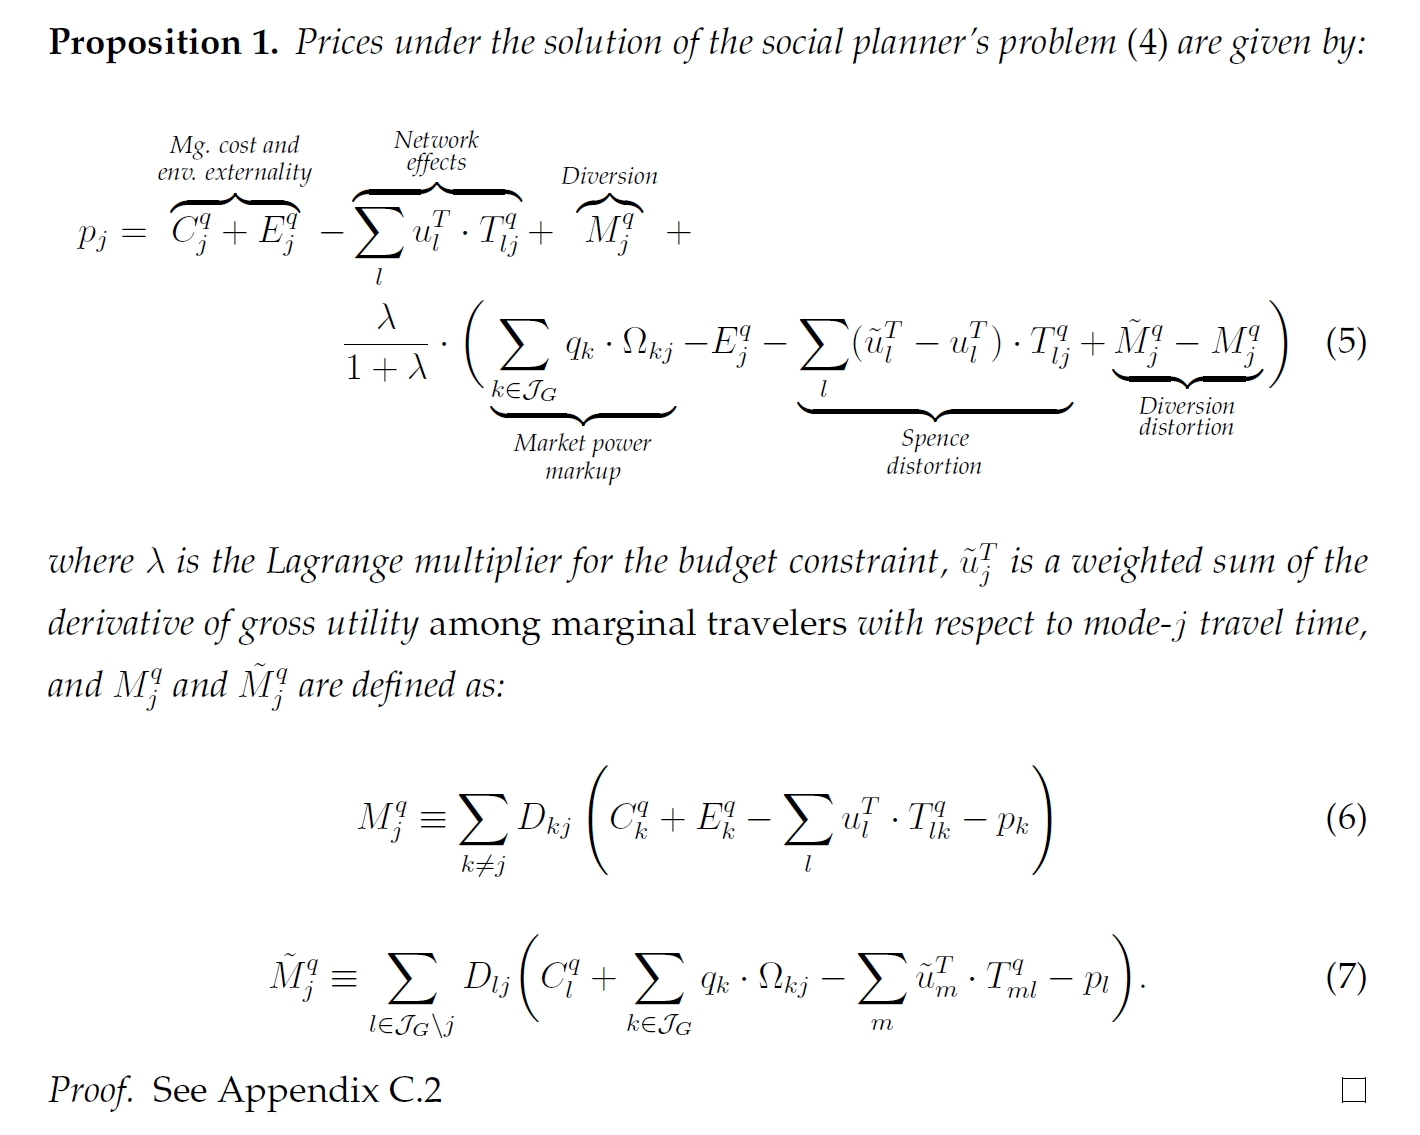
\includegraphics[width=0.66\textwidth]{../Figures/proposition1.png}
  \end{figure}
\end{frame}
\begin{frame}
  \begin{figure}
    \centering
    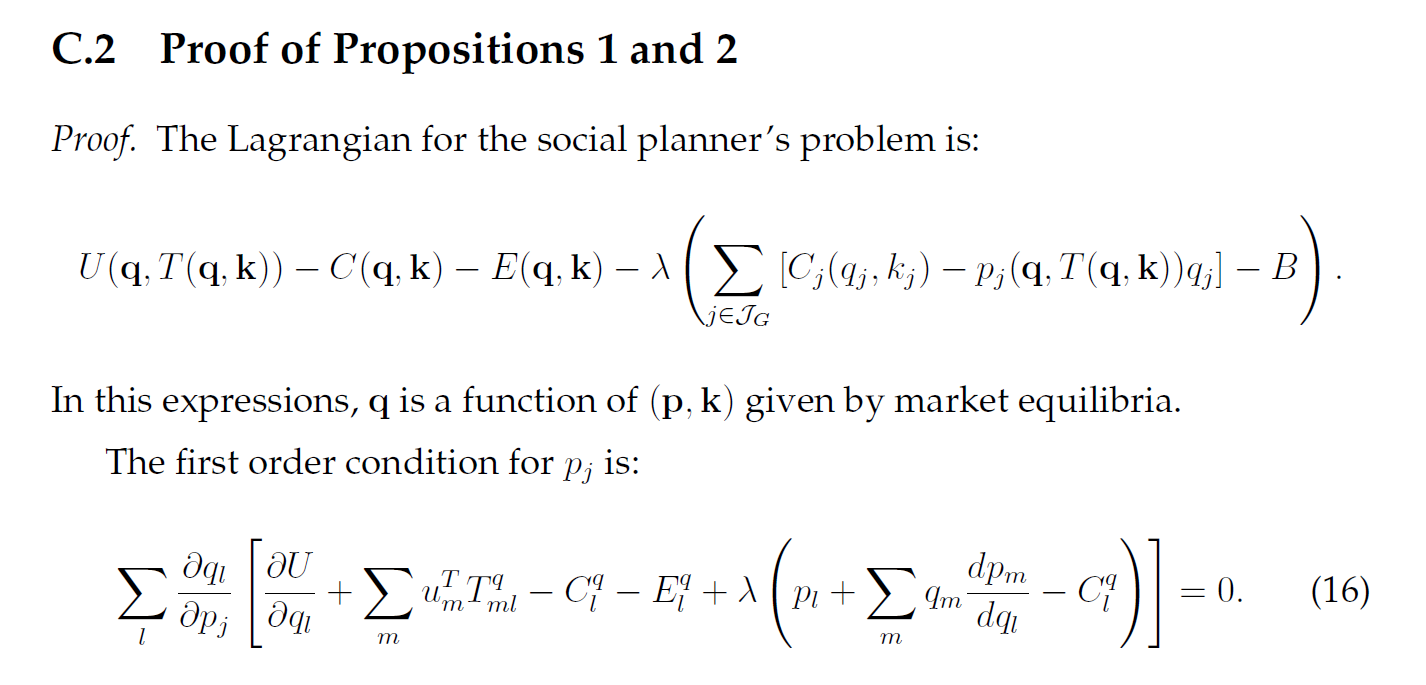
\includegraphics[width=0.66\textwidth]{../Figures/proposition1_proof.png}
  \end{figure}
\end{frame}

\begin{frame}

\end{frame}

\begin{frame}

\end{frame}

\begin{frame}{Empirical results}
  \begin{columns}[T,onlytextwidth]
    \column{0.5\textwidth}

    \begin{figure}
      \centering
      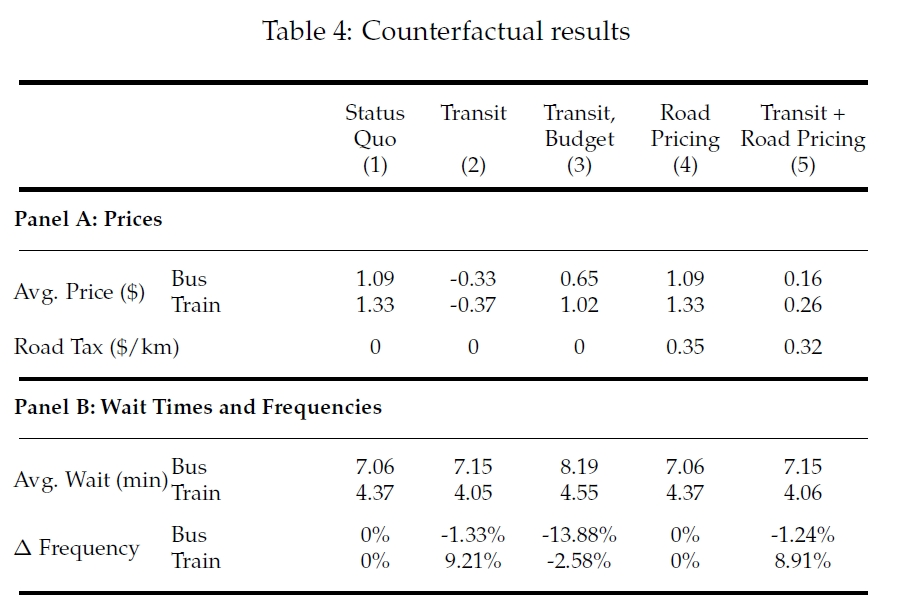
\includegraphics[width=0.9\textwidth]{../Figures/counter1.png}
    \end{figure}

    \column{0.5\textwidth}

    \begin{figure}
      \centering
      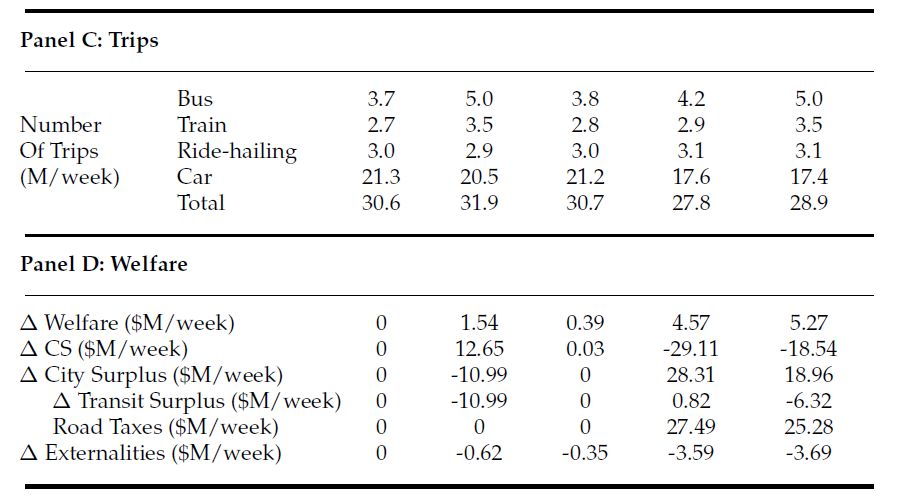
\includegraphics[width=0.9\textwidth]{../Figures/counter2.png}
    \end{figure}
  \end{columns}
\end{frame}

\begin{frame}
  \begin{figure}
    \centering
    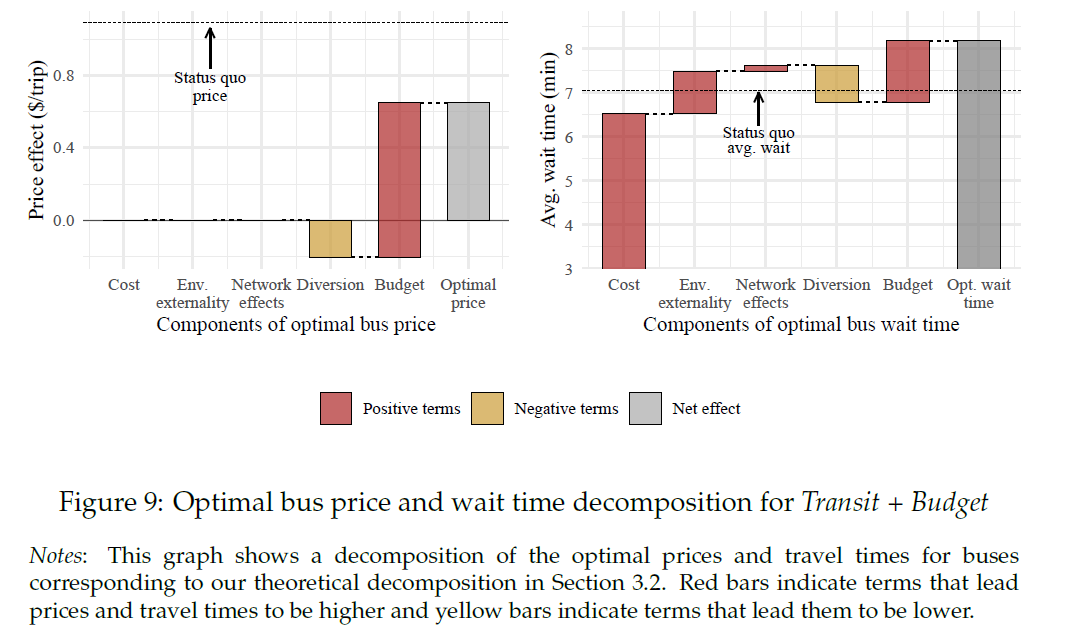
\includegraphics[width=0.8\textwidth]{../Figures/transit_budget.png}
  \end{figure}
\end{frame}

\begin{frame}
  \begin{figure}
    \centering
    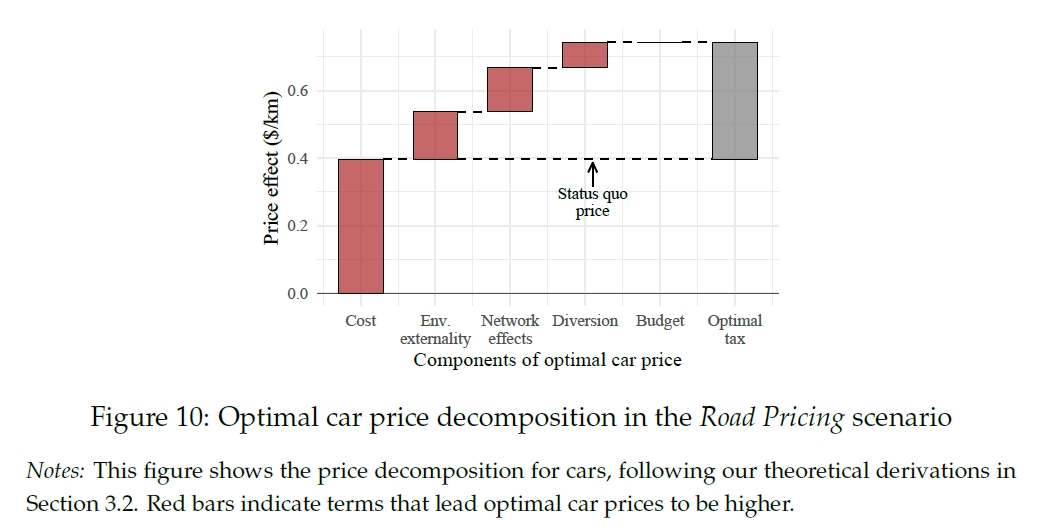
\includegraphics[width=0.8\textwidth]{../Figures/road_budget.png}
  \end{figure}
\end{frame}

\section{Conclusion}
\begin{frame}{Discussion}
  \begin{itemize}
    \item Spill over effect across different hours (market)
    \item Joint decision of outbound and inbound trips
    \item Relocation effect
    \item Route reoptimization
  \end{itemize}
\end{frame}
\begin{frame}{Conclusion}
  Government can undo the “monopoly” distortions that arise due to \textbf{budget constraint} by using road pricing revenues to \textbf{cross-subsidize} public transit.\\
  Indeed, recent transit policies in London and New York explicitly designate the revenues from road pricing to fund public transit. \textbf{Our results highlight that such
    combined policy approaches can eliminate inefficiencies.}

\end{frame}

{\setbeamercolor{palette primary}{fg=tse-red, bg=tse-pink}
\begin{frame}[standout]
  Thanks
\end{frame}
}

\appendix

\begin{frame}[allowframebreaks]{References}

  \bibliography{ref.bib}
  \bibliographystyle{apalike}

\end{frame}

\end{document}
